\documentclass{IOS-Book-Article}

\usepackage{mathptmx}
\usepackage{graphicx}
\usepackage{subfigure}

%\usepackage{times}
%\normalfont
%\usepackage[T1]{fontenc}
%\usepackage[mtplusscr,mtbold]{mathtime}

\begin{document}
\begin{frontmatter}              % The preamble begins here.

%\pretitle{Pretitle}
\title{Parallelizing Finite Element Methods Assembly for Unstructured Meshes with D\&C}
\runningtitle{D\&C Assembly}
%\subtitle{Subtitle}

\author[A]{\fnms{Lo\"ic} \snm{Th\'ebault}%
\thanks{Corresponding Author E-mail: }},
\author[A]{\fnms{Eric} \snm{Petit}},
\author[A]{\fnms{Marc} \snm{Tchiboukdjian}},
and
\author[B]{\fnms{Quang} \snm{Dinh}}

\runningauthor{L. Th\'ebault et al.}
\address[A]{PRISM - University of Versailles, France}
\address[B]{Dassault Aviation, Saint-Cloud, France}

\begin{abstract}
Current algorithms and runtimes struggle to scale to a large number of cores and show a poor parallel efficiency on current HPC machines.
Pure MPI codes are wasting IO, memory and communications. HPC users have to explore new paradigms to make an efficient usage of the shared resources,
such as hybrid MPI+threads.
In this paper we propose and evaluate a Divide \& Conquer, D\&C, approach for the parallelization on shared memory of an unstructured mesh assembly to sparse matrix.
Our target application is an industrial CFD application from Dassault Aviation.
Our implementation is based on the versatile Cilk runtime and standard MPI.
The original Fortran code has been modified with a minimum intrusion into the original pure MPI application.
Preliminary results on the matrix assembly of the application are encouraging and show good locality and scalability characteristics.
\end{abstract}

\begin{keyword}
Divide and Conquer, Task, Cilk, Mesh Partitioning, CFD, Matrix Assembly, FEM
\end{keyword}
\end{frontmatter}

\thispagestyle{empty}
\pagestyle{empty}

\section{Introduction}
%Positionment : code MPI compare to hybrid.\\
%Problem on FEM : assembling, parallelization with shared memory non trivial.\\
%Assembling on multicore, not on GPU (most of papers are for GPUs)\\\\

Current algorithms and runtimes struggle to scale to a large number of cores and show a poor parallel efficiency on current HPC machine. 
The major effects of the core count increase are a lower memory per core, higher requirement for concurrency (TLP, ILP, vector), higher coherency traffic and higher cost
for coherency protocol.
It results a severe challenge for performance scalability. The many-core accelerators such as the Xeon Phi exacerbate even more these issues.
HPC users have to explore new paradigms to make an efficient usage of the new resources. 

In order to mitigate the node scalability issues, users can modify their application using hybrid MPI + threads to take advantage of the full topology of the machine
and enhance the data and synchronization locality.
In this paper, we propose and evaluate a new parallelization strategy for structured problem based on the Divide and Conquer, D\&C, principle. Our implementation is based on a task-based runtime,
Cilk~\cite{cilk5}. 

We demonstrate the potential of the D\&C approach on the matrix assembly step from Finite Element Methods, FEM.
This step consists in building from the mesh the matrix describing a linear system of equations.
The values in the sparse matrix result from a reduction operation of some neighbor elements.
The irregularity of the structure and the sequentialization of the reduction are challenging to achieve an efficient parallelization.
For multicores, except the state of the art coloring approaches, there is very few recent works published on parallelizing matrix assembly.
In the manycore context, new algorithms are design for GPUs~\cite{cecka2011assembly,CPUGPUasm}, but can not be efficiently applied to shared multicores.

We apply our D\&C strategy for the parallelization of the matrix assembly on an industrial CFD code from Dassault Aviation computing the effect of mesh deformation
to optimize airplane structure.
Our results outperform the original pure MPI implementation and the coloring approach for shared memory parallelization.
\\\\
The paper outline is the following:
\begin{itemize}
\item Section 2 presents the matrix assembly in FEM applications using the coloring approach and our D\&C proposal using Cilk and MPI.
\item Section 3 presents related works on recent assembly approaches and uses of D\&C on FEM applications.
\item Section 4 presents the experimental setups and results of the assembly parallelization of a Dassault Aviation application, called DEFMESH.
\item Section 5 is the conclusion and presents our future works.
\end{itemize}

\section{Matrix Assembly}
%The process alterate the mesh geometry and be conservative of the mesh topology.  We have to work on a very unstructured mesh. Therefore, load balancing and interface
%computation prevent us to use geometrical domain decomposition.
%We use METIS~\cite{Metis} to do a topological domain decomposition that will not vary with the mesh deformation.
%The application iterates over three basic steps:
%\begin{itemize}
%\item Edge matrix assembly to CSR storage from the mesh coordinate array. This step potentially needs MPI communication in the case of using the elastic version.
%Explain in section ...
%\item Solve ... ??? what?
%\item Update the mesh coordinate and value, exchange the halo with other MPI rank.
%\end{itemize}

Matrix assembly is common in most of scientific applications using Finite Element Methods.
A simple assembly illustration on a 2D regular mesh is presented in figure~\ref{fig:2Dasm}.
The value on $(N1,N2)$ edge is the sum reduction the contributions of elements $E1$ and $E2$.
In 3D, the number of neighbor elements can be arbitrary large.

Because of the reduction step and the frontier sharing resulting of the domain decomposition, this step is non trivial to parallelize.
To create parallelism, one must create independent domains to work on and synchronize between them to handle frontier elements.
In that case we envision two different approaches, a state-of-the-art coloring approach and our proposition of D\&C based on a topological recursive bisection.
\begin{figure}[htp]
 \centering
 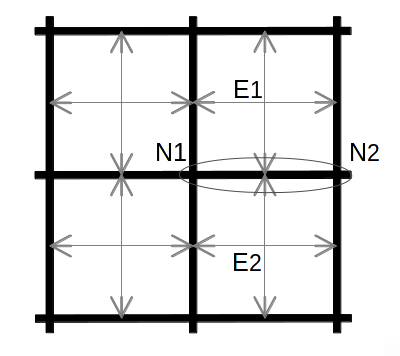
\includegraphics[scale=0.2]{2D_asm.png}
 \caption{2D assembling example}
 \label{fig:2Dasm}
\end{figure}

\subsection{Coloring}
\label{sec:col}
Coloring avoids race conditions by assigning a different color to elements sharing an edge.
It was originally targeting vectorial machines because all elements of a same color are independent and thus their contribution can be vectorized.
Determining a minimal coloring is NP-complete, but create a coloring with an undefined number of color is relatively simple~\cite{findsomeonetocite}.
A pseudo-code and a simple 2D coloring example are given in figure~\ref{fig:colApp}.

\begin{figure}[htp]
 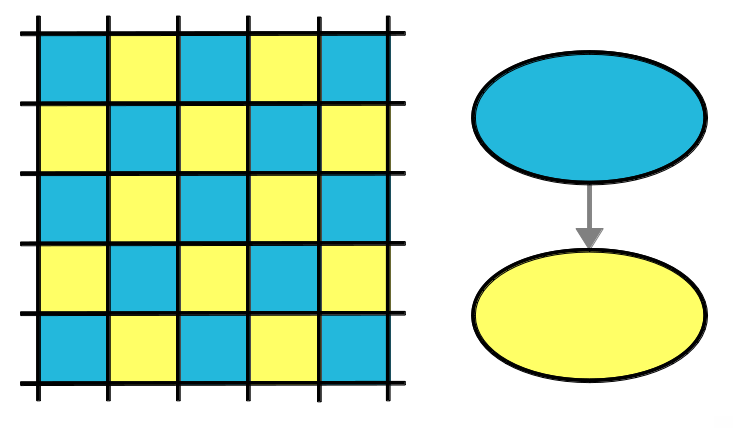
\includegraphics[scale=0.2]{Coloring_approach.png}
 \begin{verbatim}
From initial Element_to_Node array {
    create Node_to_Element array
    create Element_to_Element array
    create Element_to_Color array
    create Color_to_Element array
}
For each color - in sequential
    For all elements of current color - in parallel
        Compute element contribution
 \end{verbatim}
 \caption{Coloring approach}
 \label{fig:colApp}
\end{figure}

Despite coloring is an efficient approach for vectorial machines, it is not well suited for current shered memory parallel architectures.
When sorting the elements by color, we improve the spatial locality and allow the vectorization. However there is only one update per edge per color and each color runs over all the domain  before going to the next one. Thus there will probably be no locality between colors.


\subsection{Divide \& Conquer}
%D\&C, approach on  unstructured meshes
%%
%The D\&C approach is particularly interesting for its ability to scale naturally to an increasing number of node thanks to its architecture oblivious concept.
%Each leaves is responsible of its own data and there is a very minimal amount of sharing, avoiding costly locks and coherency protocols. 

The main idea of the D\&C approach for shared memory parallelization is to create task level parallelism while preserving a good data locality and minimizing synchronization cost.
Instead of increasing MPI domain decomposition and communications with the data size increases, we increase the number of Cilk tasks and threads. MPI processes remain
in moderate numbers. This way, we take benefit of the machine topology and most of communications are replaced by data sharing.

The rational is to divide recursively the work in two or more independent tasks, synchronize locally these tasks before returning. This recursive approach has many advantages.
First the recursive sharing naturally exposes high concurrency. As long as the application is large enough, it is possible to produce a deeper tree to get more concurrency and 
therefore match the higher requirement of many-core system. Furthermore synchronization are local: only nodes of a same parent node in the recursive
tree needs to be synchronized. And finally, it greatly improved the data locality by reordering the data in smaller independent sets. 

On a small number of cores,  The scalability of the D\&C parallelization is expected to be equivalent to the pure MPI, but on a larger number of cores, we expect to continue scaling
while pure MPI should not. In any case the code will benefit from the higher locality and reuse of elements in the D\&C version and all the versions using the reordering should outperform the original code.

This approach is decomposed in two parts described in following subsections.
First part is a recursive decomposition of each MPI domain and second part is the recursive execution of the assembly step using Cilk.

\subsubsection{Recursive Bisection}
\label{sec:DCrec}
D\&C is based on a topological recursive bisection of the mesh.
As illustrated in figure~\ref{fig:DCapp}, the left and right sub-domains created by these bisections are not sharing any element and thus, can be executed in parallel.
However, the separator elements in the middle have nodes in both sides and must be treated after left and right sub-domains.

The load-balancing between the subdomain is really important since it influence the depth of the recursive tree. Having a balanced tree will minimize the maximum depth and thus the number of synchronization on the critical path. On the other side, the size of the frontier which cannot not be processed in parallel of the left and right domain directly impact the parallel efficiency.
Therefore it is important to use a good partitioner to build equal sub-domains while minimizing the interface. In our case, we use the METIS graph partitioner~\cite{Metis}.

In order to increase the data locality, we also permute node and element arrays.
Indeed, nodes and elements can be consecutive in memory inside each sub-domain, improving intra-task locality.
Secondly, since the tasks distribution is following the recursive domain decomposition, we store neighbor sub-domains and associated separator contiguously
to improve locality between tasks.
These permutations are applied in all MPI domains, therefore we renumber the nodes on the interface so that exchanged data stay consistent.
\begin{figure}[htp]
 \centering
 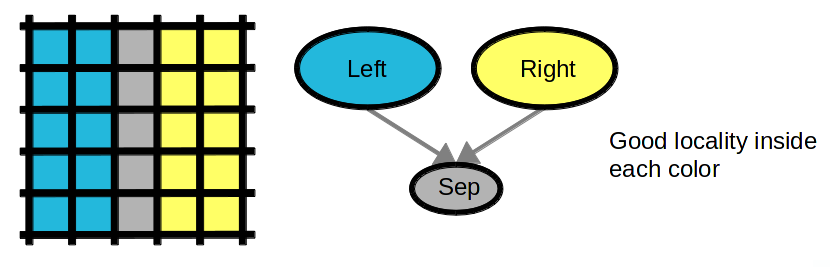
\includegraphics[scale=0.17]{DC_approach.png}
 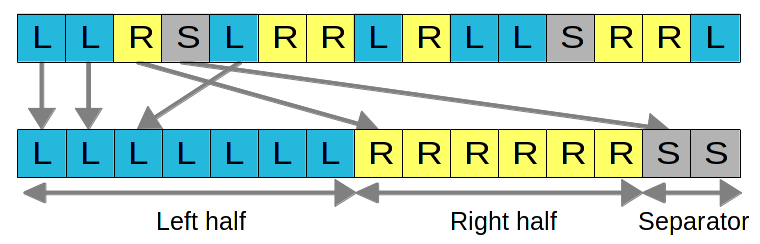
\includegraphics[scale=0.21]{Data_permutations.png}
 \caption{D\&C approach}
 \label{fig:DCapp}
\end{figure}

This approach is then applied recursively to all sub-domains, offering a large amount of parallelism.
As illustrated in figure~\ref{fig:DCrec}, each leaf of the resulting tree is associated to an independent Cilk task and executes the matrix assembly on its sub-domain.
In order to optimize the locality with permutations without multiplying tasks, it is possible to stop the recursionbefore reaching the leaves. To do so the task execute in one block the left, right and sep arator domain which are stored contiguously in memory.

The partitionment is topological: cuts are done on edges rather than geometrical coordinates.
This allows to compute sub-domains only one time for a mesh, and it is independent from the rest of the computation. Therefore this partition is precompute and stored with the mesh.
During the run, the application needs only to apply the precomputed permutations before executing the recursive assembly.
\begin{figure}[htp]
 \centering
 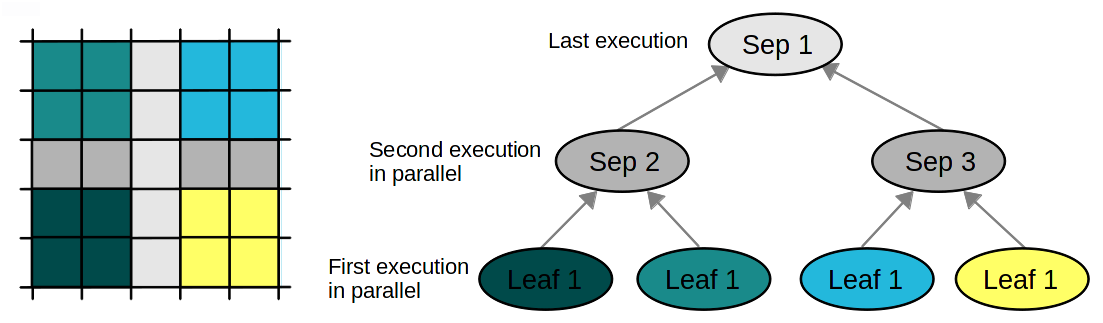
\includegraphics[scale=0.25]{DC_recursion.png}
 \caption{D\&C recursive execution}
 \label{fig:DCrec}
\end{figure}

\subsubsection{Cilk Implementation}
Cilk~\cite{cilk5} is a task based runtime originally developed by Frigo, Leiserson and Randal at MIT and now supported by Intel.
It allows to \emph{spawn} and \emph{sync}hronize many parallel tasks.
All these tasks are stored in queues and executed by \emph{worker} threads.
In order to improve the load balancing, Cilk runtime uses a work-stealing scheduler. When a \emph{worker} completes its queue, it can steal additional tasks from
slower \emph{workers}.

Starting from the tree shown in figure \ref{fig:DCrec}, the Cilk implementation is then straightforward.
While the recursion has not reached a leaf (domain size condition), left and right sub-domains of each node are split in two tasks and executed in parallel. Whe then wait these hasks to complete before launching the separator computation. 
When the recursion reaches the leaves, the original sequential assembly code is executed on the subdomain.
A pseudo-code for this recursion is given in figure~\ref{fig:DCcode}.

In other section of an application, when all elements are accessed in a regular loop, there is no need to use a recursive task tree. In that purpose Cilk provides, as well as OpenMP, an easy way to parallelize loops using the \emph{cilk\_for} keyword. By simply substituting the original \emph{for} by this keyword, iterations of the loop are split recursively in several parallel tasks. Thanks to the reordering of the element, the \emph{cilk\_for} will also beenficiate of the D\&C locality. On the DEFMESH application, we observe a better scalability with the \emph{cilk\_for} than with \emph{OpenMP parallel for} pragma.
\begin{figure}[htp]
 \begin{verbatim}
foo (sub-domain) {
    if Node is not a leaf
        spawn foo (sub-domain.left)
        foo (sub-domain.right)
        synchronize
        foo (sub-domain.sep)
    else
        sequential assembly (sub-domain)
}
 \end{verbatim}
 \caption{D\&C assembly pseudo-code}
 \label{fig:DCcode}
\end{figure}

\section{Related Works}
Many choices are available to complete FEM assembly in parallel.
All methods have their advantages and their limitations, depending for instance on the target architecture or the mesh size.

Recent studies~\cite{cecka2011assembly,CPUGPUasm} investigates different ways to compute FEM assembly on CPUs and GPUs.
The method of "TODO with one?"~\cite{} consists in creating parallelism between all the non-zero entries of the system of equations.
This method has a very fine grain parallelism and thus, applies only to GPUs. They then store contributions from all mesh elements to global or local memory in parallel, and then reduce in parallel these contributions to compute the non-zero values.
By arranging the data layout, this method can offer good performances on GPUs.
However, it can suffer of load imbalancing since the number of element contributors for computing non-zero values is heterogeneous.
Moreover, it is very memory consuming and thus limited to small test cases.
Another variant consists in using one thread for the whole assembly step of one non-zero value at a time, but this approach leads to redundant computations of element
contributions.
The method presented in~\cite{} consists in assembling by mesh element. One thread is responsible for the whole assembly step of one element at a time. It can be applied to both GPUs and CPUs.

A coloring approach~\cite{CUDAfe,CPUfe} can be used to launch several threads in parallel on independent elements.
This way each thread has a good load balancing per color. The load balancing between colors has no influence since they are sequentialized.
However, it can suffer from poor performances because of a bad data locality as explained is section~\ref{sec:col}.

Mtrix assembly approach for Recursive Sparse Blocks (RSB) matrix on CPUs has also been experimented~\cite{RSBasm}. Despite this format can offer good results in solver algorithms~\cite{RSBsolver}, assembly on RSB matrix seems to be highly memory-bandwidth bound~\cite{RSBasm}.

In 2008, Dongarra et al. experiments important benefits on CPUs by implementing an asynchronous tasks based parallelism approach on well-known factorization algorithms
compare to traditional fork-join approach~\cite{Dongarra}.
A recent investigation on hybrid programmation integrating task base parallelism in MPI processes have been made~\cite{MPIhybid}.
The experiments done on a 1024 nodes cluster result in significant speed-up on several micro-benchmarks and strong scaling applications compared to pure MPI.

\section{Experiments}
To validate our approach, we apply the D\&C algorithm using Cilk and MPI on a the assembly step of an application from Dassault Aviation called DEFMESH.
We compare our results to the original pure MPI version of the assembly step and also to a MPI + OpenMP version using the coloring approach.

\subsection{Dassault Aviation DEFMESH Application}
The DEFMESH application is a Computational Fluid Dynamics (CFD) code based on a Finite Element Method (FEM).
It is used to apply deformations on an initial mesh in order to optimize its fluid flows.
It is fully parallelized with the MPI protocol and recently with OpenMP in few parts of the solver.
This solver is based on a conjugate gradient method and is mainly composed of dot products, SpMVs and reductions.

DEFMESH main kernel is decomposed in three steps.
First one is the assembly step where mesh data are gathered into a CSR structure.
Second step is the solver step which works on this CSR structure and computes optimal displacements.
Final step is the update of mesh coordinates using previously computed deformations.

Two versions of the kernel exist, the laplacian and the elastic version. Elastic version has a more complex assembly step and different boundary conditions for the solver.
While a simple scalar is computed for each edge of the mesh in the Laplacian version, a 3 by 3 matrix based on a more complex equation is computed in the elastic version.
Moreover, both versions can be whether linear or non linear.
The linear versions compute displacements in one step of deformation using the conjugate gradient methods as a direct method.
In the non linear versions, the deformation is split into a given number \emph{N} of smaller deformations.
The mesh is updated after each deformation and thus, each step of the kernel are repeated $N$times. The solver is then used as an iterative method.

We launch this application on two different test cases which are both unstructured meshes from Dassault Aviation.
First one is a small mesh of 152 086 elements and 27 499 nodes which represents an M6 wing. We used it for developing and debugging.
Second test case, called EIB, is composed of 6 346 108 elements and 1 079 758 nodes. It represents the displacement of fuel tank along a plane fuselage.
This EIB test case has been used for experiments and measures presented in next section.

\subsubsection{To do}
nice picture of mesh deformation comparing variants\\

\subsection{Experimental Setups}
Experiments are done on the Dassault Aviation EIB test case. EIB is an unstructured mesh composed of 6 346 108 elements and 1 079 758 nodes. It represents the displacement of a fuel tank along a plane fuselage. This case is illustrated in the figure~\ref{TODO:add the figure from quang report}

In the following experiments, we compare two versions of the DEFMESH application: the original one from Dassault Aviation called $Ref$ and the new Divide \& Conquer
version called $D\&C$.
The original version uses MPI between the different blocks of the mesh and OpenMP in some loops of the solver.
The D\&C version, as described above uses a recursive partitioning of each block of the mesh. It exploits, in addition to MPI and OpenMP,
a Cilk task parallelism of the assembly step.
We also compare our results to the coloring implementation of the assembly, using OpenMP parallelism.

For each of these versions, we consider the Laplacian and elasticity variants of DEFMESH.
For both of them, the application runs in 50 steps of resolution and measures correspond to the average time of one iteration.
In all cases we measure the assembly step, where the D\&C approach has been applied.
We also measure the solver to estimate the impact of the data permutations on the rest of the code.

We present the results both in terms of execution times and of parallel efficiency.
In all the graphics, the X axis represents the number of cores used. It corresponds to the product of MPI processes by the number of threads.
In graphics presenting execution times, the Y axis correspond to RDTSC cycles for the assembly step and to MPI\_Wtime seconds for the solver.
Concerning efficiency, the Y axis represents the parallel efficiency given by the following formula:
$E_{P} = \frac{T_{S}}{P*T_{P}}$. $E_{P}$ is the efficiency on $P$ processor, $T_{S}$ the sequential time, and $T_{P}$ the time on $P$ processors.

For each graphics, we use 1, 4, 8 and 12 MPI tasks and from 1 to 12 threads while the combination of MPI processes per threads is lower or equal to 12.
This corresponds to the number of cores available. In all cases, the number of Cilk threads used in the assembly is equal to the number of OpenMP threads used in the solver.
We also varied the number of METIS partitions and Cilk tasks in a large scope of values but we have not observed significant changes in the results.
Final values are 512 partitions and 128 Cilk tasks. This corresponds to approximately 10 tasks per core, which is recommended in Cilk documentations. TODO and enough to fit into caches?

All experiments have been done with default policies. The OpenMP affinity is set to scatter and Cilk threads are not pinned.
These experiments runs on an UVSQ server composed of twelve cores distributed in two sockets of 6-cores Intel® Xeon® X5650 clocked at 2.67 GHz.
Concerning memory hierarchy, each core has its own L1 and L2 caches of resp. 32KB and 256KB and a shared L3 cache of 12MB. Main memory is split in two NUMA nodes of 16GB.

\subsection{Results}

The following sections presents our measurement for the elastic and laplacian version for the FEM assembly. 

NOTE TO REVIEWER: The experiments on coloring are in progress and will be included in the final version of the paper

\subsubsection{Assembly}
As we can see in figures~\ref{fig:asmCurvesA} and~\ref{fig:asmCurvesC}, with a low number of cores of work the D\&C approach is slower than pure MPI, especially when we increase
the number of cores.
This is due to the remaining sequential part of the D\&C code.
Indeed, separator elements are not parallelized and can represent an important proportion of the computation.
According to the Amdahl law, by increasing the number of cores, the proportion of the sequential part increases. This is confirmed on figure~\ref{fig:asmCurvesC} showing the parallel efficiency.

In the elasticity variant, illustrated in figures~\ref{fig:asmCurvesB} and~\ref{fig:asmCurvesD}, the D\&C approach becomes equivalent to the pure MPI.
Since the amount of work of the assembly step is bigger than in the laplacian variant, the proportion of the sequential computation, including the separators, is lower. In this case the scalability improves. Furthermore, contrary to the pure MPI version, the data always fits in L2 cache with the D\&C version.

Unlike the original version that makes irregular accesses to the cells of the matrix, the D\&C version works on matrix cells packed contiguously in small sub-matrix corresponding to the Cilk tasks.
For any problem size, with D\&C, we can increase the number of partitions such that the tasks working-set will always fit in cache.

To conclude, these first results are encouraging and we can reasonably expect to match the ideal scaling when the separators will be parallelized.

\begin{figure}[htp]
 \centering
 \subfigure[Laplacian execution time]{\label{fig:asmCurvesA}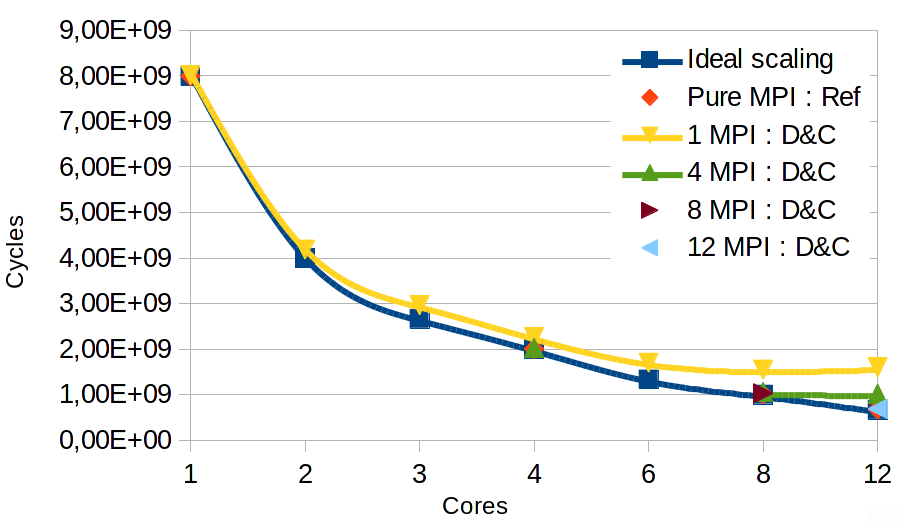
\includegraphics[width=0.49\textwidth]{Laplacian_asm_time.png}}
  \subfigure[Laplacian parallel efficiency]{\label{fig:asmCurvesC}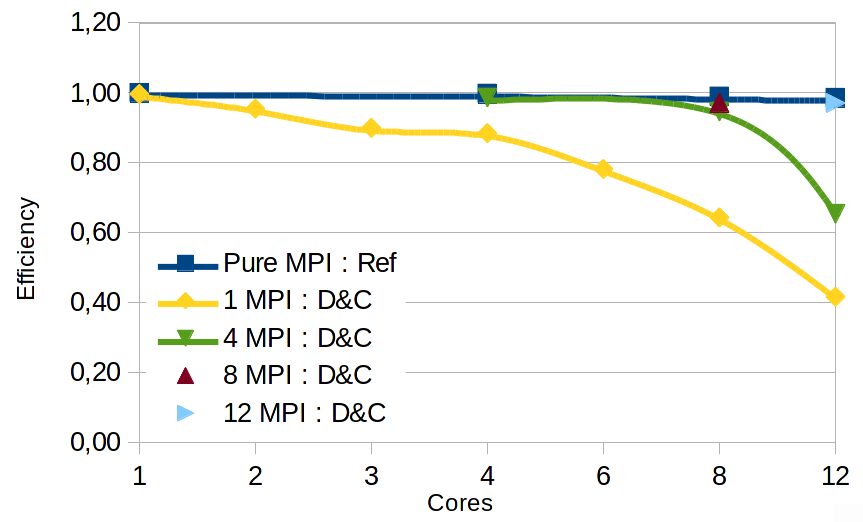
\includegraphics[width=0.49\textwidth]{Laplacian_asm_efficiency.png}}
 \subfigure[Elasticity execution time]{\label{fig:asmCurvesB}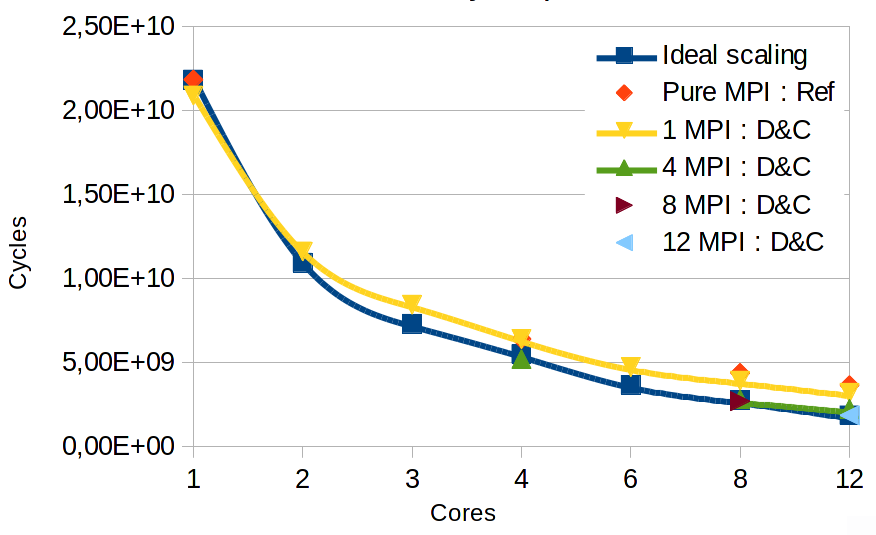
\includegraphics[width=0.49\textwidth]{Elasticity_asm_time.png}}
 %\hspace{1em}
 \subfigure[Elasticity parallel efficiency]{\label{fig:asmCurvesD}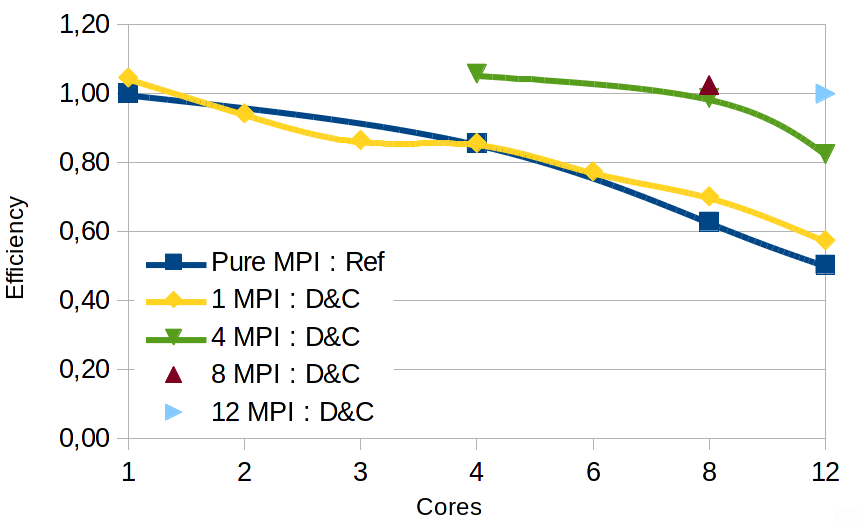
\includegraphics[width=0.49\textwidth]{Elasticity_asm_efficiency.png}}
 \caption{Assembly measures}
 \label{fig:asmCurves}
\end{figure}

\subsubsection{Solver}
Despite we did not modify the solver part, we observe approximately 6\% benefit of the D\&C version compared to the reference version.
This gain is due to the better data locality enabled by the permutations explained in section~\ref{sec:DCrec}. To show the impact of locality, we randomly permute the data and observe a degradation of the performance. We then measure the L3 cache misses occurring in the solver for the original version and the D\&C permutted version. They are 23\% lower with D\&C.

\begin{figure}[htp]
 \centering
 \subfigure[Laplacian]{\label{fig:solCurvesA}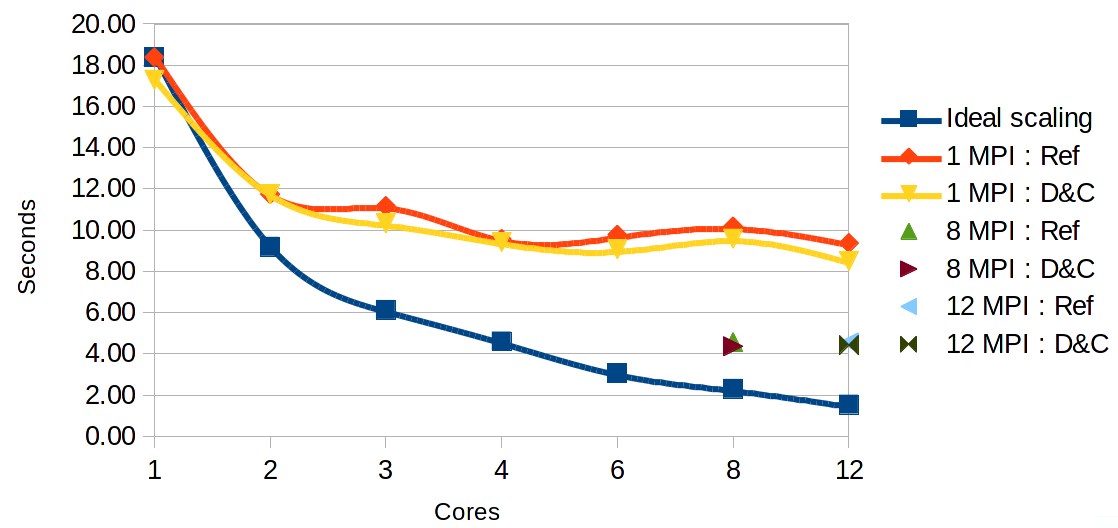
\includegraphics[scale=0.158]{Laplacian_solver_time.png}}
 \subfigure[Elasticity]{\label{fig:solCurvesB}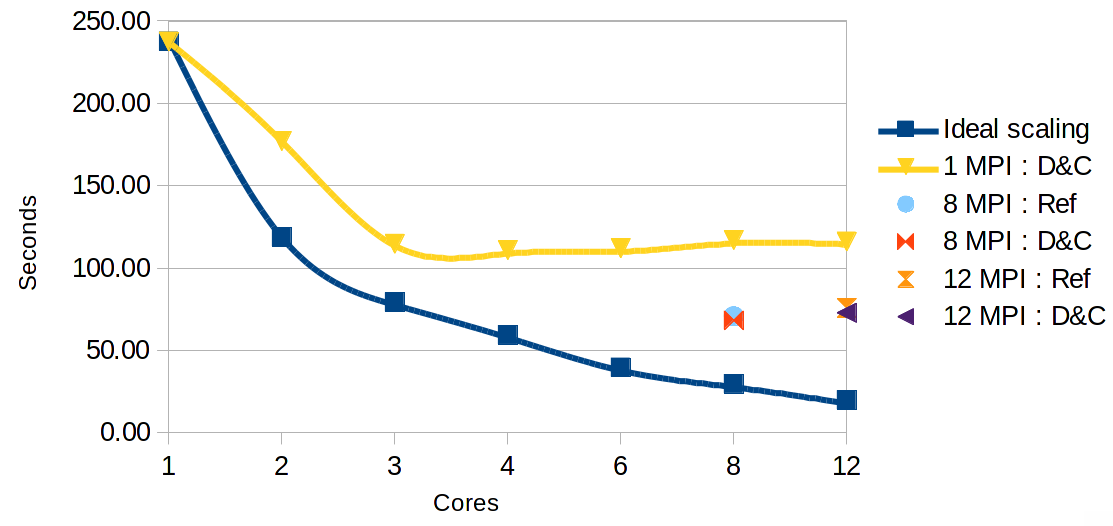
\includegraphics[scale=0.154]{Elasticity_solver_time.png}}
 \caption{Solver execution time}
 \label{fig:solCurves}
\end{figure}

\section{Conclusion and Future Work}
FEM assembly is the first step of many applications, such as seismic simulation, metal forming, or crash test simulations. Depending on the application, the FEM assembly can cover more than 80\% of the execution time.
In the Dassault Aviation DEFMESH application, our current implementation is already faster than the pure MPI original version and overpasses in performance and scalability the state-of-the-art coloring approach.

Even without exploiting the thread level parallelism, the D\&C approach  significantly improves the locality and the scalability and execution time. The pure MPI version with D\&C has a perfect strong scaling for our experimental setup.

As a future work, we plan to parallelize the separator in the D\&C FEM assembly and experiment on a larger number of cores.
We strongly believe that our approach will provide good performances on new manycores such as Xeon Phi. Extension will focus on D\&C friendly data structure definition and apply D\&C on other parts of the FEM application. 
%We are also considering a hybrid approach using coloring inside each D\&C sub-domains in order to enable vectorization.
\bibliographystyle{unsrt}
\bibliography{dc_bib}

\end{document}